Considerando o modelo conceitual, os requisitos funcionais e não-funcionais, partiu-se para a elaboração do modelo entidade-relacionamento para este contexto. O modelo entidade-relacionamento atuará como um esquema conceitual para o banco de dados da aplicação a ser desenvolvida, incluindo os detalhes dos tipos de entidade, relacionamentos e restrições, mas abstraindo detalhes de implementação \cite{Navathe:Livro}.

Como resultado, obteve-se o modelo entidade-relacionamento apresentado na Figura \ref{fig:mer}. É possível notar uma semântica bastante similar ao modelo conceitual apresentado na seção anterior, o que é desejável. Este modelo entidade-relacionamento apresentado foi fielmente seguido na ocasião da implementação da solução proposta.

\begin{figure}[H]
	\centering
	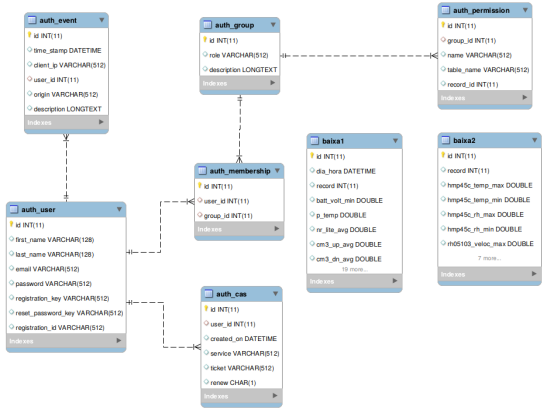
\includegraphics[scale=1.0]{img/mer.png}
	\caption{Módelo Entidade Relacionamento - LabInstru Web.}
	\label{fig:mer}
\end{figure}
